%*****************************************
\chapter{Der Graphen Generator}\label{ch:generierung}
%*****************************************
Nun beschäftigt sich diese Arbeit im weiteren damit, wie typische soziale Netzwerke generiert werden können. 
Zunächst bietet es sich an dieser Stelle oftmals an, da Facebook und Instagram der Informationspflicht unterliegen, seine eigenen social Media Daten anzufordern. Meist spiegelt dieser Datensatz gelikete und kommentierte Posts der Nutzer*innen wieder, oder verfasste Nachrichten und gesuchte Inhalte.
Bei den ersten Visualisierungsversuchen wird bereits klar, dass diese Daten für eine wissenschaftliche Arbeit nicht brauchbar sind, da es sich bei den erstellten Plots und Ergebnissen nicht um \textit{ typische soziale Netzwerke} aus Tabelle \ref{TableEigenschaften} handelt. Vielmehr bestehen diese meist aus einem Kernknoten, also einem sogenannten sternförmigen Graphen. Plots wie Abbildung \ref{fig:OwnData} sind bei der Visualisierung der eigenen Daten entstanden. Diese besteht aus unzähligen einzelnen Teilgraphen, welche lediglich eine weitere Verbindung aufweisen. Auch sind keine Cliquen oder Brücken in solchen Graphen zu finden, was ebenfalls dafür spricht, dass es sich um kein \textit{typisches soziales Netzwerk} handelt. \\
\FloatBarrier
\begin{figure}[h!]
    \centering
    %\hspace*{-1cm}
    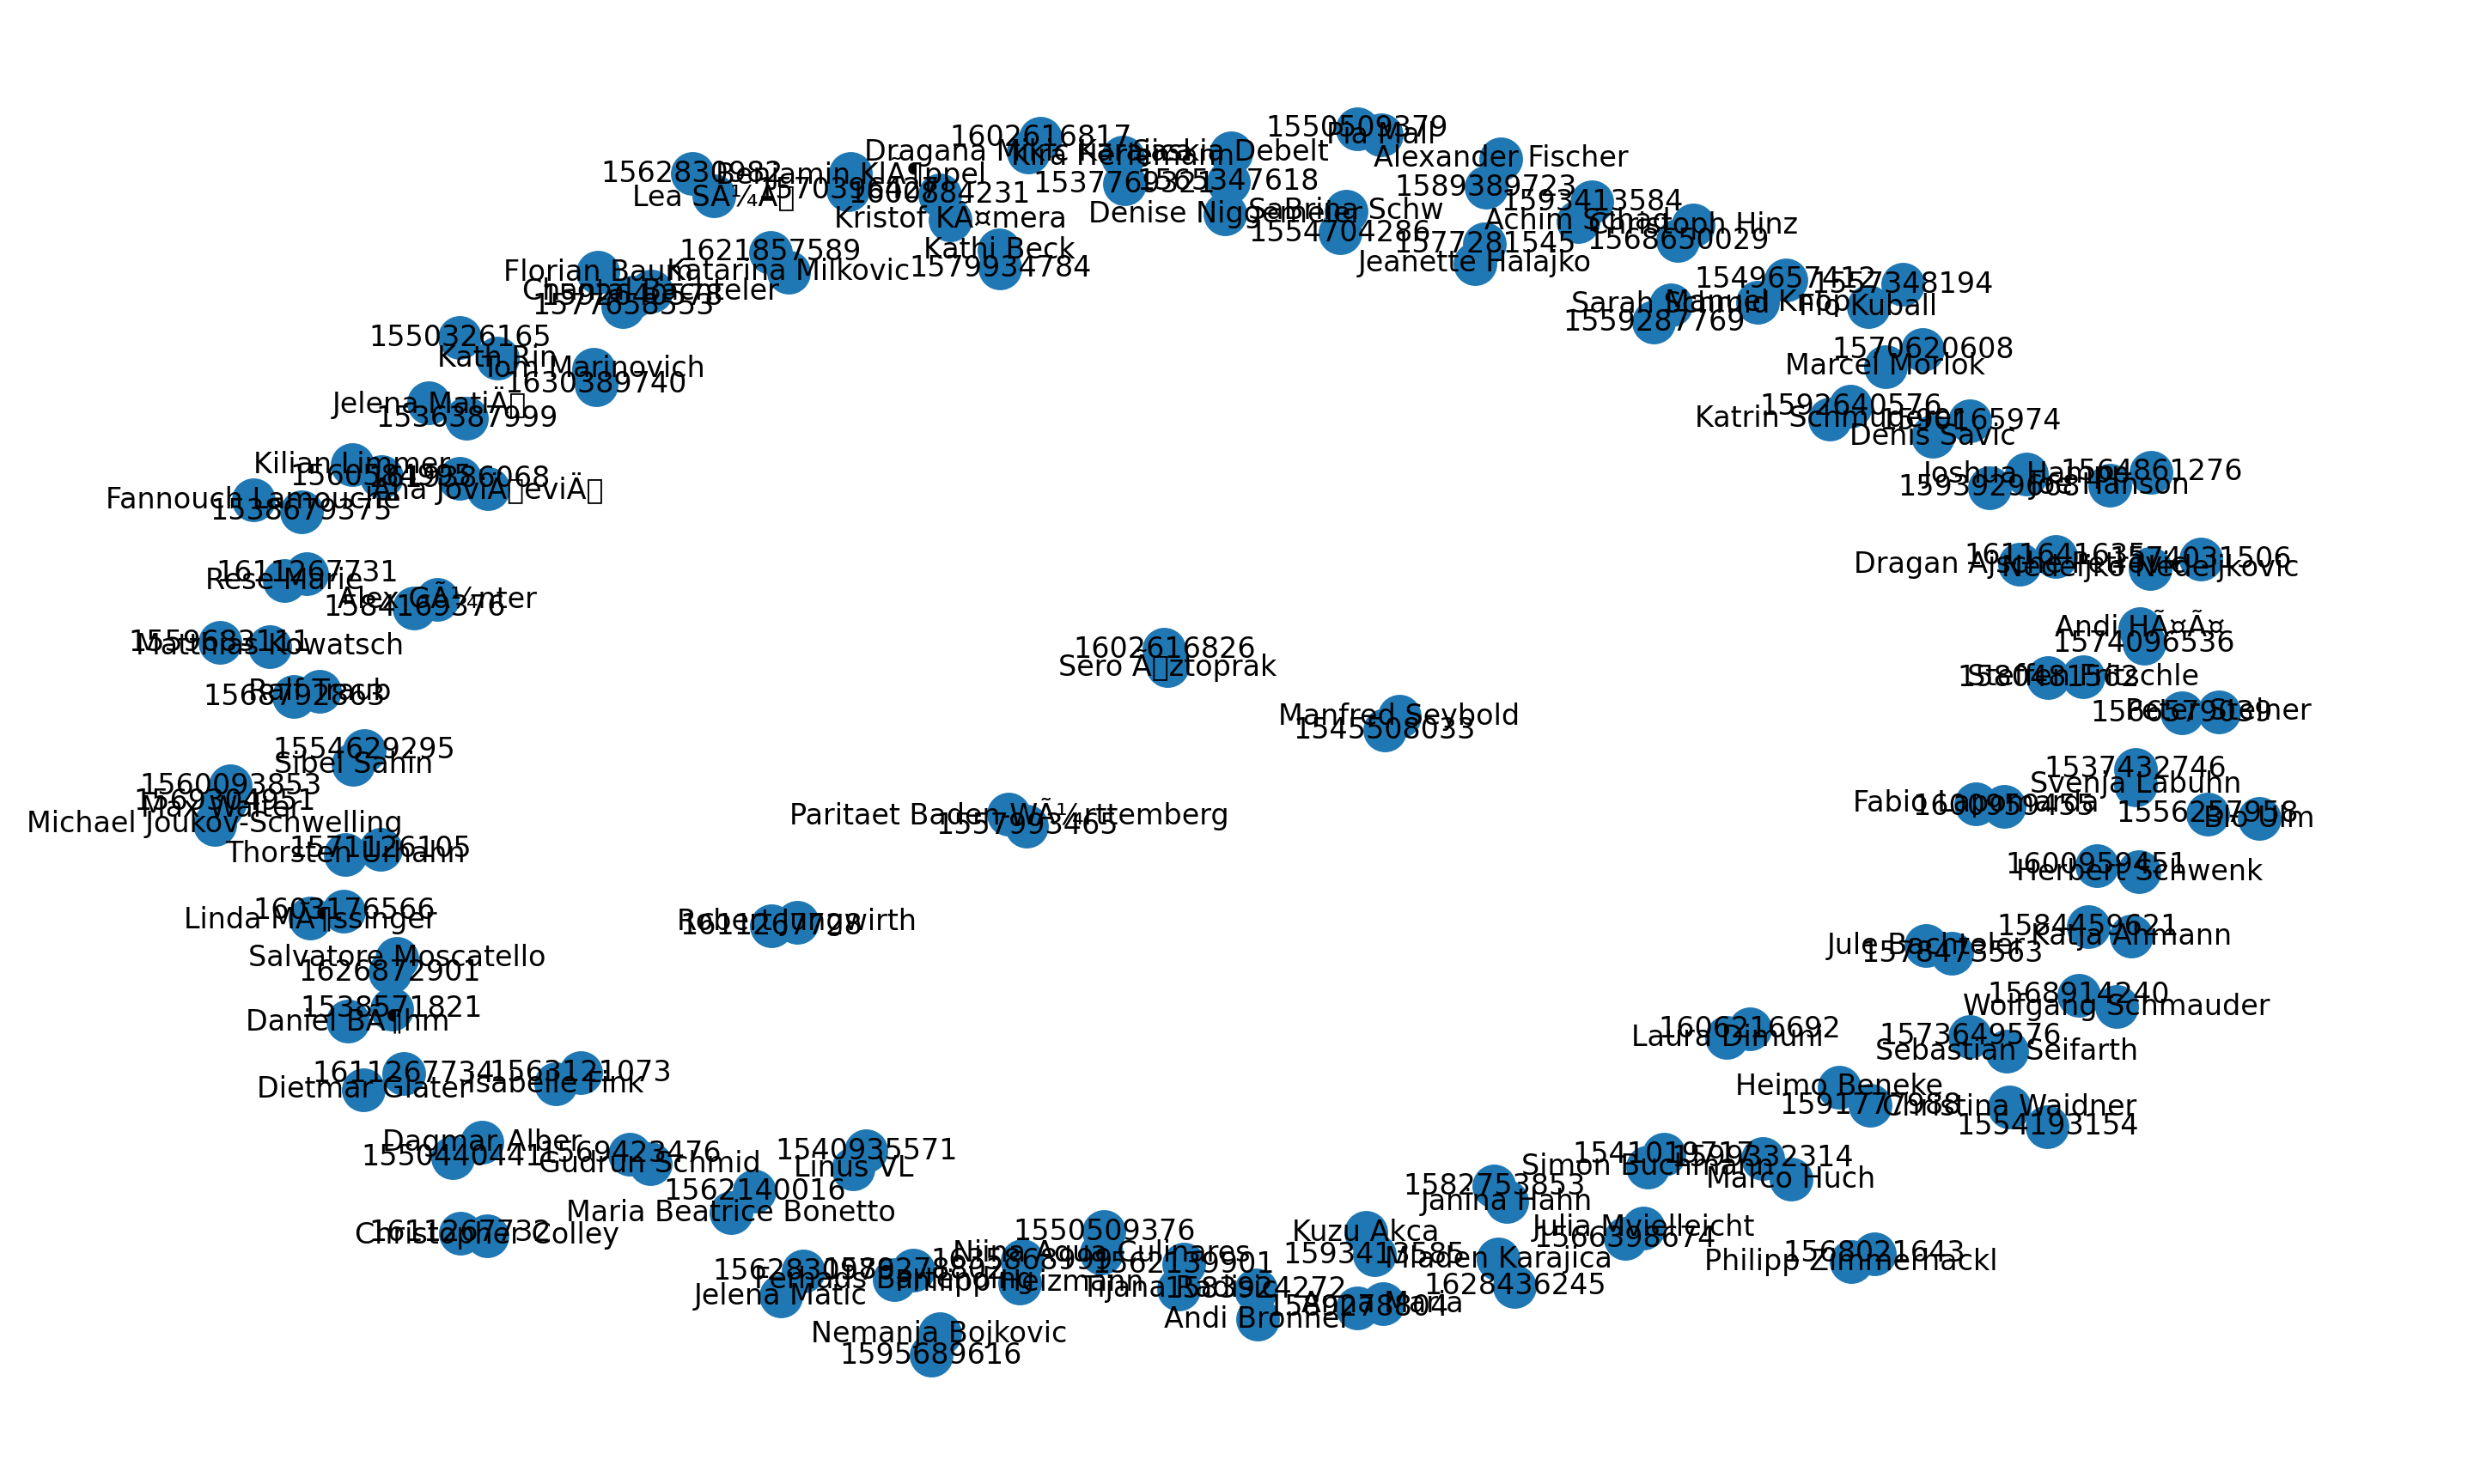
\includegraphics[width=0.7\textwidth]{Graphics/PlotOwnData.png}
    \caption{Erste Versuche eines Sozialen Netzwerks, \\
    selbst erstellt}
    \label{fig:OwnData}
\end{figure}
\FloatBarrier

Eine weitere Schwierigkeit ist bei diesen Graphen die Interpretation der Kanten, denn diese ist teilweise nicht eindeutig. 
Facebook gibt lediglich IDs bekannt, doch welche Bedeutung diese haben ist unbekannt aber im Endeffekt auch nicht relevant für diese Arbeit.

\section{Generierung eines sozialen Netzwerks} 
Bei einer endlichen Anzahl von Knoten \textit{n} gibt es auch eine endliche Anzahl von möglichen Graphen, die aus diesen Knoten erzeugt werden können. Hierbei wächst die Anzahl der Graphen mit \textit{n} Knoten exponentiell.
Ein Zufallsgraph ist nur einer dieser Graphen, der durch einen Zufallsprozess erzeugt werden kann.
Wenn von \textit{Zufallsgraphen} die Rede ist, wird in den meisten Fällen das \textit{Erdős-Rényi-Modell} als Graphengenerator verwendet (benannt nach den Mathematikern Paul Erdős und Alfréd Rényi). Eine wichtige Eigenschaft von, auf diese Weise erzeugten Zufallsgraphen ist, dass alle Konstellationsmöglichkeiten des Graphen gleichverteilt erzeugt werden \cite{Generators}.
Neben dem Erdős-Rényi-Modell, gibt es noch viele weitere Methoden zur zufälligen Netzwerkmodellierung \cite{Generators}.
\begin{itemize}
    \item Die \textit{dense$\_$gnm$\_$random$\_$grap-Modellierung} liefert einen Zufallsgraphen.
    Bei dem Modell wird ein Graph gleichmäßig zufällig aus der Menge aller Graphen mit einer gegebenen Anzahl an Knoten und Kanten ausgewählt.
    \item Bei der \textit{Newman–Watts–Strogatz small-world graph-Modellierung} wird zunächst ein Ring mit $n$ Knoten erzeugt. Dann wird jeder Knoten im Ring mit seinen $k$ nächsten Nachbarn verbunden (oder $k - 1$ Nachbarn, wenn $k$ ungerade ist). Anschließend wird für jede Kante im Ring mit $k$ nächsten Nachbarn, mit der Wahrscheinlichkeit $p$, eine neue Kante hinzugefügt.
    \item Die \textit{random$\_$regular$\_$graph-Modellierung} gibt einen zufälligen regulären Graphen mit $n$ Knoten zurück. Das heißt, alle Knoten besitzen gleich viele Nachbarn als somit den selben Grad.
    Der resultierende Graph hat keine Selbstschleifen oder parallele Kanten.
    \item Die \textit{barabasi$\_$albert$\_$graph-Modellierung} hingegen liefert einen Zufallsgraphen nach dem Barabási-Albert-Präferenzmodell.
    Ein Graph mit $n$ Knoten wird durch Anhängen neuer Knoten mit jeweils $m$ Kanten erzeugt, die bevorzugt an bestehende Knoten mit hohem Grad angehängt werden.
    \item Die \textit{powerlaw$\_$cluster$\_$graph-Modellierung} ist im Wesentlichen das\\ Barabási-Albert-Wachstumsmodell mit dem zusätzlichen Schritt, dass für jede zufällige Kante die Chance besteht, dass ebenfalls eine Kante zu einem seiner Nachbarn besteht (und damit ein Dreieck entsteht) \cite{Generators}.
\end{itemize}

\FloatBarrier
\begin{figure}[h!]
    \centering
    \hspace*{-1.5cm}
    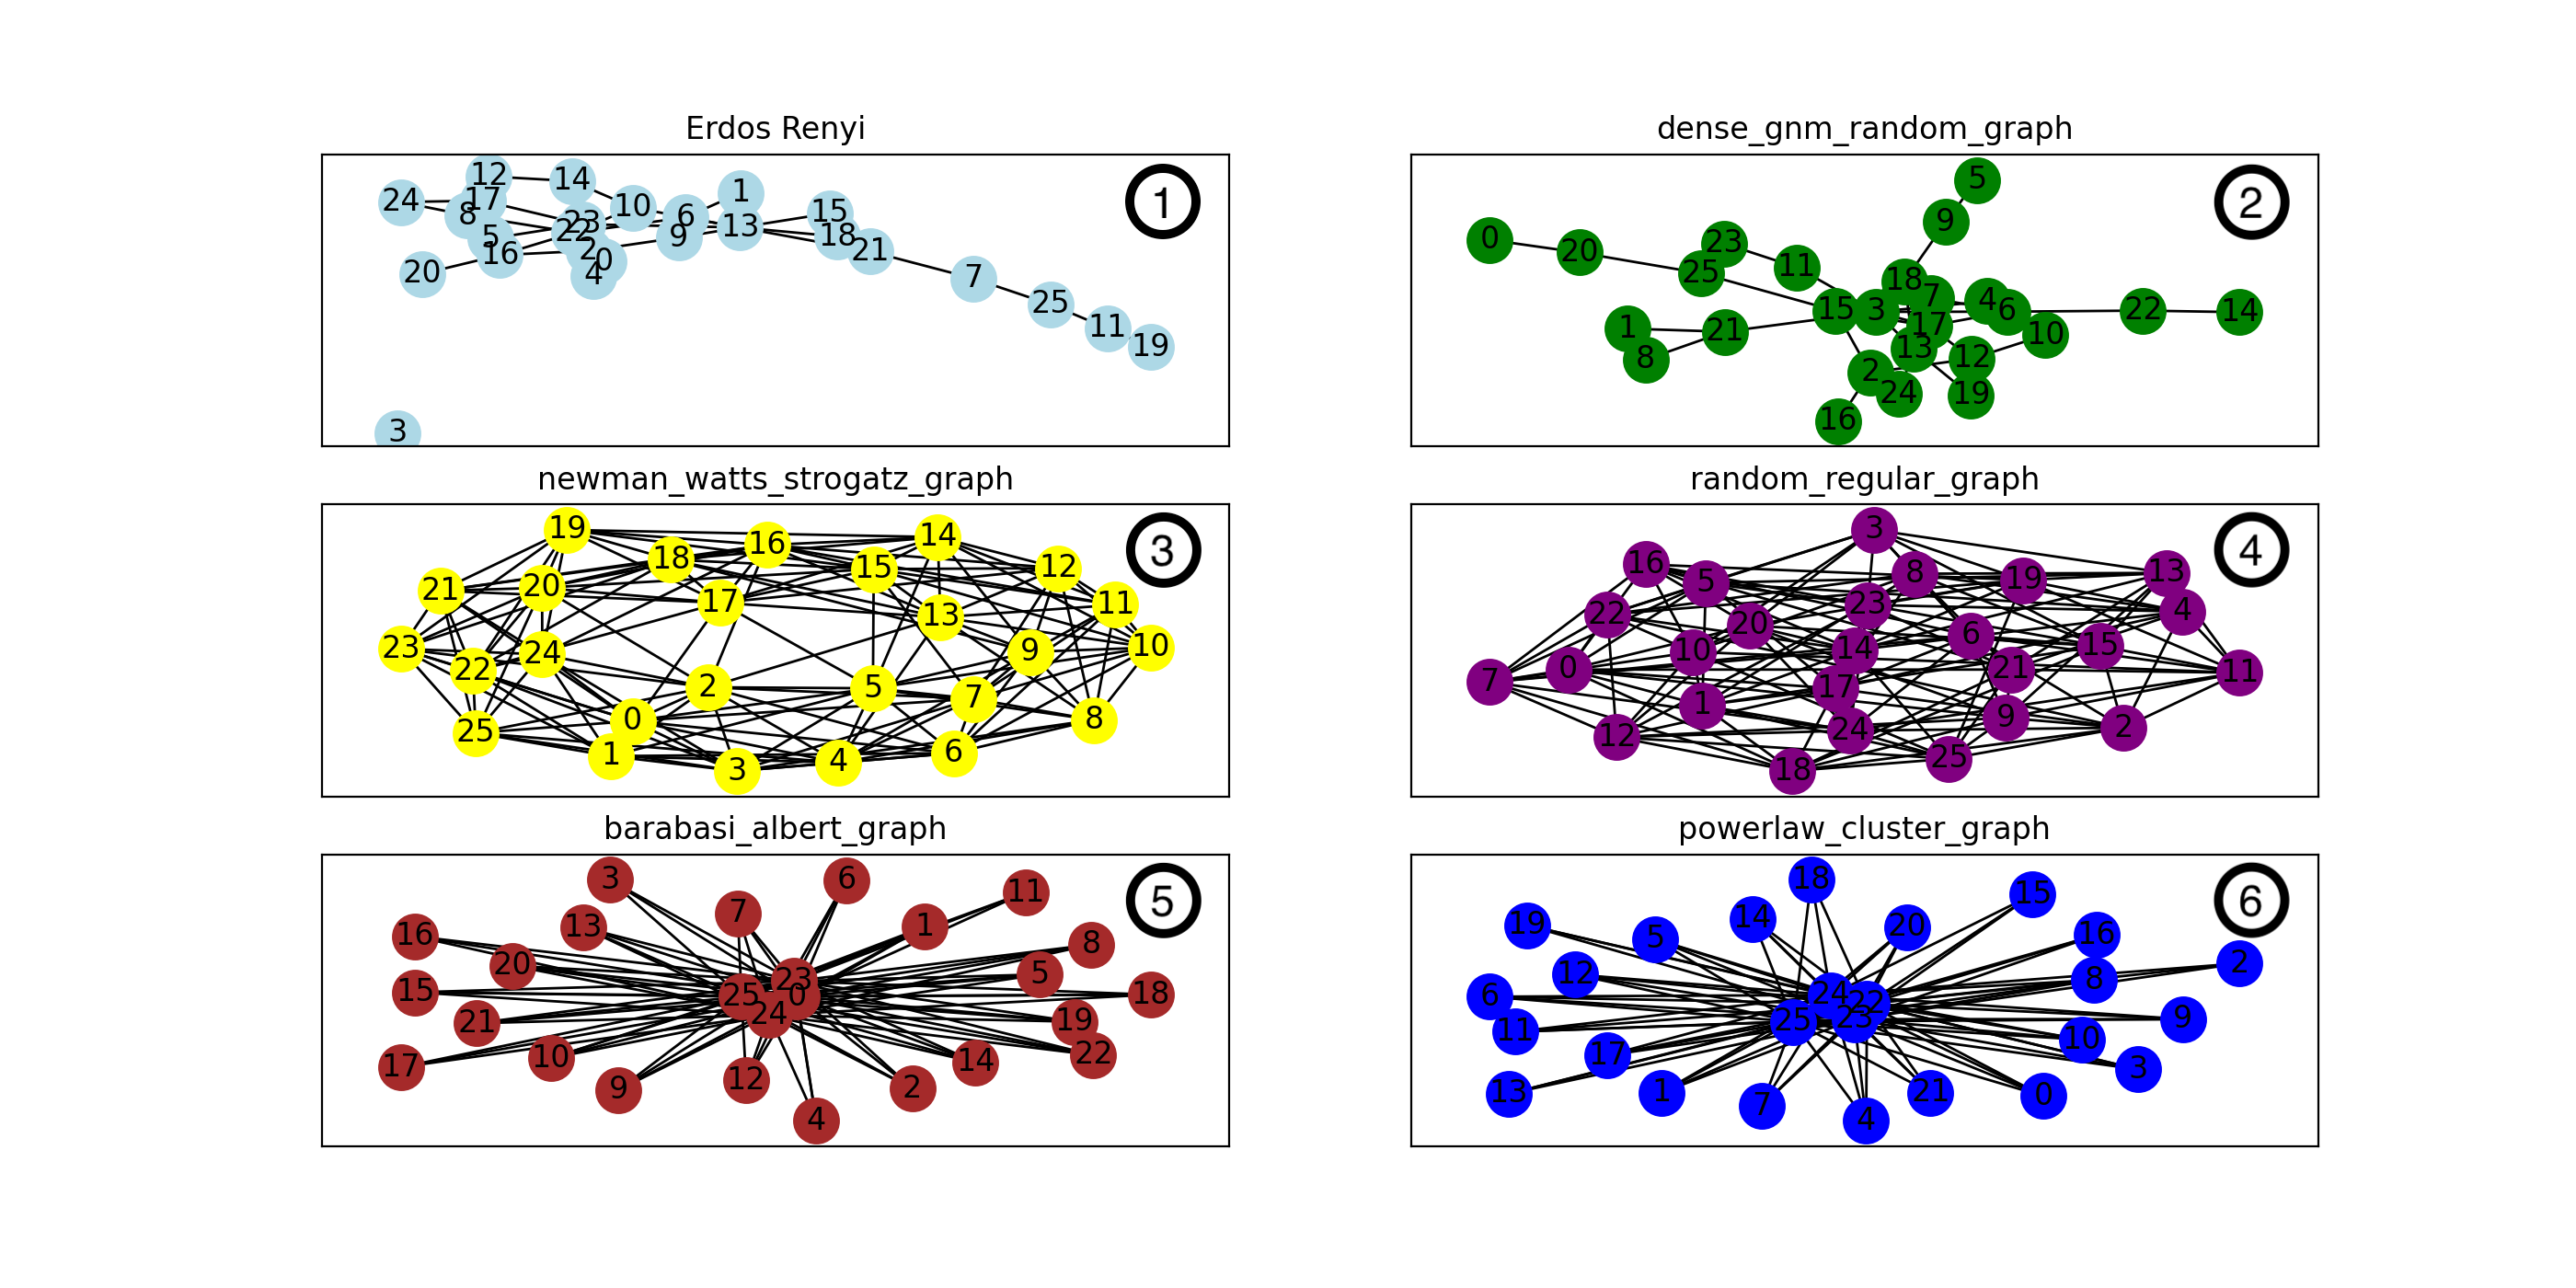
\includegraphics[width=1.2\textwidth]{Graphics/6Random.png}
    \caption{Zufällig erstellte Graphen mit 25 Knoten entsprechend der jeweiligen Methoden}
    \label{RandomGraphen}
\end{figure}
\newpage

Bei den Graphen in Abbildung \ref{RandomGraphen} wurde lediglich eine visuelle Interpretation durchgeführt und nicht die Graphen mit den jeweiligen Zentralitäten analysiert. Auf den ersten Blick erkennen wir, dass bei allen sechs Modellen Unstimmigkeiten zu typischen Eigenschaften von \textit{sozialen Netzwerken} aus Tabelle \ref{TableEigenschaften} auftreten. Beispielsweise bei dem \textit{Barabasi Albert Graph} und dem \textit{Powerlaw cluster graph} (\textbf{5} und \textbf{6}) sind einzelne zentrale Knoten zu erkennen. Diese zentrale Knoten sind von vielen weiteren Knoten umgeben, die alle wiederum mit diesen zentralen Knoten verbunden sind. Es sind also keine Cliquen und auch keine Cluster zu erkennen. Auch der \textit{newman watts strogatz graph} und der \textit{random regular graph} (\textbf{3} und \textbf{4}) entsprechen nicht den erwünschten \textit{sozialen Netzwerken}. Bei beiden Plots scheint es, als sei jeder Knoten mit jedem weiteren Knoten verbunden, was erneut eine untypische Eigenschaft ist. Es existiert also nur lediglich eine große Clique. Nun bleiben noch die beiden Plots des \textit{Erdos Renyi-Graphen} und \textit{dense gnm random graph} (\textbf{1} und \textbf{2}), welche ebenfalls nicht unseren Erwartungen entsprechen. Der Plot des \textit{dense gnm radom graph} weist zwar einzelne Äste auf, doch generell wenige Cliquen enthalten und keine Cluster aufweist, weshalb dieses Modell ebenfalls nicht brauchbar ist. Bei dem \textit{Erdos Renyi Modell} besteht die gleiche Problematik wobei hier noch das Problem hinzu kommt, dass ein isolierter Knoten existiert. Ein isolierter Knoten ist ein Knoten der keinen Nachbarn besitzt, also Grad $0$ aufweist.
Dies würde beispielsweise auf Sozial Media, bezogen bedeuten, dass Nutzer*innen auf dieser Plattform angemeldet sind, die keinerlei Verbindungen besitzen. Dies kann durchaus der Fall sein, es ist aber sehr unwahrscheinlich, dass Menschen auf solchen Plattformen angemeldet sind und keinerlei Freunde haben oder andere Nutzer*innen folgen.
\newpage
Schließlich kommt bei den oberen zwei Modellen noch dazu, dass bereits visuell betrachtet kaum Cliquen und auch keine Brücken auffindbar sind. Deshalb muss auch bei diesem Modell kritisch hinterfragt werden, ob es sich bei den Graphen um ein \textit{typisches soziales Netzwerke} handeln könnte. Deshalb liegt nahe, dass Anpassungen durchgeführt werden müssen.\\


Eine mögliche Adaption wird erzielt, indem von den zufälligen Graphen-Methoden, die im vorherigen Abschnitt eingeführt wurden, abgewichen wird. Eine weitere Überlegung wäre, alle Formeln selbständig zu implementieren und nicht die bereits vordefinierten Funktionen zu verwenden. Zum Einen sind diese vordefinierten Funktionen intransparent und daher auch fehleranfälliger, aber auch der Zugriff auf diese ist nicht ganz einfach. \\
Für die Generierung eines \textit{sozialen Netzwerks} wird unter anderem eine Methode benötigt, die einzelne zufällige Graphen erstellt. Diese zufälligen Graphen sollen am Ende die jeweiligen Cluster darstellen, welche durch Brücken miteinander verbunden sind. Dadurch wären die ersten Eigenschaften eines typischen sozialen Netzwerks aus Tabelle \ref{TableEigenschaften} erfüllt.

\begin{algorithm}
\caption{Random Adjazenzmatrix}\label{randomAdjacency}
\begin{algorithmic}[1]
\Procedure{random adjacency matrix}{}
\State $\textit{matrix} \gets \text{zufällige Matrix der Größe (n,n) zufällig befüllt mit Werten zwischen 0 und 1}$
\For {alle \textit{i} in matrix}
\State befülle die Diagonale der Matrix mit 1
\For {alle \textit{i und k} in matrix}
\State setze die Wahrscheinlichkeit \textit{prob} auf einen zufälligen Wert zwischen 0 und 1
\If{\textit{matrix} an der Stelle [i][k] größer als \textit{prob}}
\State setze \textit{matrix} an dieser Stelle auf 0
\Else 
\State setze diese Stelle auf 1
\EndIf
\EndFor
\EndFor
\For {alle \textit{i} in \textit{matrix}}
\State was für \textit{matrix} an der Stelle [i][j] gilt, muss auch für [j][i] gelten
\State \textbf{RETURN} \textit{matrix}
\EndFor
\EndProcedure
\end{algorithmic}
\end{algorithm}

Der Algorithmus \ref{randomAdjacency} erstellt zufällige Matrizen, die aber erst noch zu einer großen Matrix zusammengefügt werden müssen. Die zufälligen einzelnen Matrizen sind die Cluster beziehungsweise Teilgraphen des sozialen Netzwerks. Doch wollen wir diese Cluster nun zu einem großen Graphen beziehungsweise einer großen Matrix zusammenführen. Hierfür benötigt man die Methode \textit{Graph appender}. Der Algorithmus \ref{GraphAppender} dieser Methode soll wie folgt aussehen: 

\begin{algorithm}
\caption{alle Subgraphen zu einer Liste zusammenführen}\label{GraphAppender}
\begin{algorithmic}[1]
\Procedure{graph appender}{}
\State $\textit{graphs} \gets \text{leeres Array}$
\State $\textit{n} \gets \text{Anzahl an Subgraphen / Matrizen}$
\For {alle \textit{i} zwischen 1 und \textit{n}}
\State $\textit{k} \gets \text{zufälliger integer, Größe des Subgraphen}$
\State \textbf{goTo} \text{Algorithm 1 mit dem übergebenen Wert \textit{k}}
\State \text{füge random Matrix in \textit{graphs} ein} 
\State \textbf{RETURN} \textit{graphs}
\EndFor
\EndProcedure
\end{algorithmic}
\end{algorithm}

\newpage
Die einzelne Matrizen werden der dynamischen Datenstruktur (Liste) hinten angehängt.
Nachdem nun eine Liste mit vielen zufällig erzeugten Matrizen generiert ist, fehlt lediglich eine Methode, um die Graphen zusammenzuführen und sicherzustellen, dass die Teilgraphen miteinander durch Brücken verbunden sind. Wir wollen also insgesamt sicherstellen, dass durch die Algorithmen \ref{randomAdjacency}, \ref{GraphAppender} und \ref{uniteGraphs} einzelne zufällige Subgraphen erstellt werden, die mithilfe des \textit{graph appenders} zu einer Liste zusammengeführt werden und nun über Brücken Verbindungen zueinander gebildet werden. Der Algorithmus \ref{uniteGraphs} sieht wie folgt aus:

\begin{algorithm}
\caption{Graphs zusammenführen}\label{uniteGraphs}
\begin{algorithmic}[1]
\Procedure{unite graphs}{}
\State $\textit{graphs} \gets \text{Graph aus Algorithm \ref{GraphAppender}}$
\If {\text{\textit{graphs} aus nur einem Element besteht}}
\State \text{gebe \textit{graphs} zurück}
\EndIf
\State $\textit{dim} \gets \text{0}$
\State $\textit{big graph} \gets \text{Graph mit Nullen befüllt}$
\For{alle \textit{i} zwischen \textit{0} und der Länge von \textit{graphs}}
\State $\textit{Variable a} \gets \text{zufälliger integer zwischen 0 und Länge von graphs}$
\State $\textit{Variable b} \gets \text{zufälliger integer zwischen 0 und Länge von graphs}$
\For{alle \textit{j und k} zwischen \textit{0} und \textit{graphs}}
\State $\textit{l} \gets \text{summierte Länge von \textit{graphs} bis zur Stelle i}$
\State $\textit{graph} \gets \text{\textit{graphs} an der Stelle \textit{i}}$
\\
\State $\text{in den Zeilen 16 und 17 werden die einzelnen Cluster in \textit{big graph} eingefügt}$
\\
\State $\text{\textit{big graph} an der Stelle [(l+j)][(l+k)]} \gets \text{graph[j][k]}$
\State $\text{\textit{big graph} an der Stelle [(l+k)][(l+j)]} \gets \text{graph[k][j]}$
\\ 
\State $\text{in den Zeilen 21 und 22 werden die einzelnen Cluster durch Brüken verbunden}$
\\
\State $\text{\textit{big graph} an der Stelle [(l+a)][(l+b+graphs Länge an [i]) modulo dim]} \gets \text{1}$
\State $\text{\textit{big graph} an der Stelle [(l+b+graphs Länge an [i]) modulo dim)][(l+a)]} \gets \text{1}$
\EndFor
\EndFor
\\
\\
\textit{nun wird der Knoten mit der höchsten Gradzentralität gesucht}\\
\State $\textit{counter 1} \gets \text{0}$
\State $\textit{counter 2} \gets \text{0}$
\State $\textit{Knoten} \gets \text{0}$
\For{\textit{i und j} zwischen \textit{0} und der Länge von \textit{graphs}}
\If{\textit{graphs} an der Stelle [i][j] ungleich \textit{0}}
\State $\textit{counter 1} \gets \text{erhöhe um 1}$
\If{\textit{counter 1} größer \textit{counter 2}}
\State $\textit{counter 1} \gets \text{counter 2}$
\State $\textit{Knoten} \gets \text{i}$
\EndIf
\EndIf
\EndFor
\textbf{RETURN} \textit{Knoten}
\EndProcedure
\end{algorithmic}
\end{algorithm}

\newpage
Jetzt ist ein großer Graph generiert, bestehend aus vielen zufälligen kleinen Graphen, welche durch den Knoten mit den meisten ein- und ausgehenden Kanten mit einem weiteren Subgraphen verbunden sind. Dieses Vorgehen ist aber nicht in einem der drei Algorithmen \ref{randomAdjacency}, \ref{GraphAppender} oder \ref{uniteGraphs} beschrieben, sondern im Git Repo \cite{TZ} zu finden. 
Nach weiteren Überlegungen, wie es möglich wäre, den generierten Graph noch mehr sozialen Netzwerken ähneln zu lassen und die Eigenschaften aus Tabelle \ref{TableEigenschaften} zu erfüllen, ist zusätzlich die Idee entstanden eine Methode zu schreiben, die sicherstellt, dass der generierte Graph aus einer bestimmten Anzahl an Cliquen besteht. Mit diesem zusätzlich Faktor soll sichergestellt werden, dass der generierte Graph mehr Kanten besitzt als davor, um die Wahrscheinlichkeit für eine existierende Clique zu erhöhen. Der Cliquen-Methode, die ebenfalls im Git Repo \cite{TZ} zu finden ist, soll hierfür eine fixe Zahl $n$ übergeben und zusätzlich sichergestellt werden, dass stetig neue Graphen generiert werden, bis die Anzahl an Cliquen genau der fixen Zahl $n$ entspricht.
Durch die Algorithmen \ref{randomAdjacency}, \ref{GraphAppender} und \ref{uniteGraphs} entsteht schließlich folgender Graph:

\FloatBarrier
\begin{figure}[h!]
    \centering
    \hspace*{-1.5cm}
    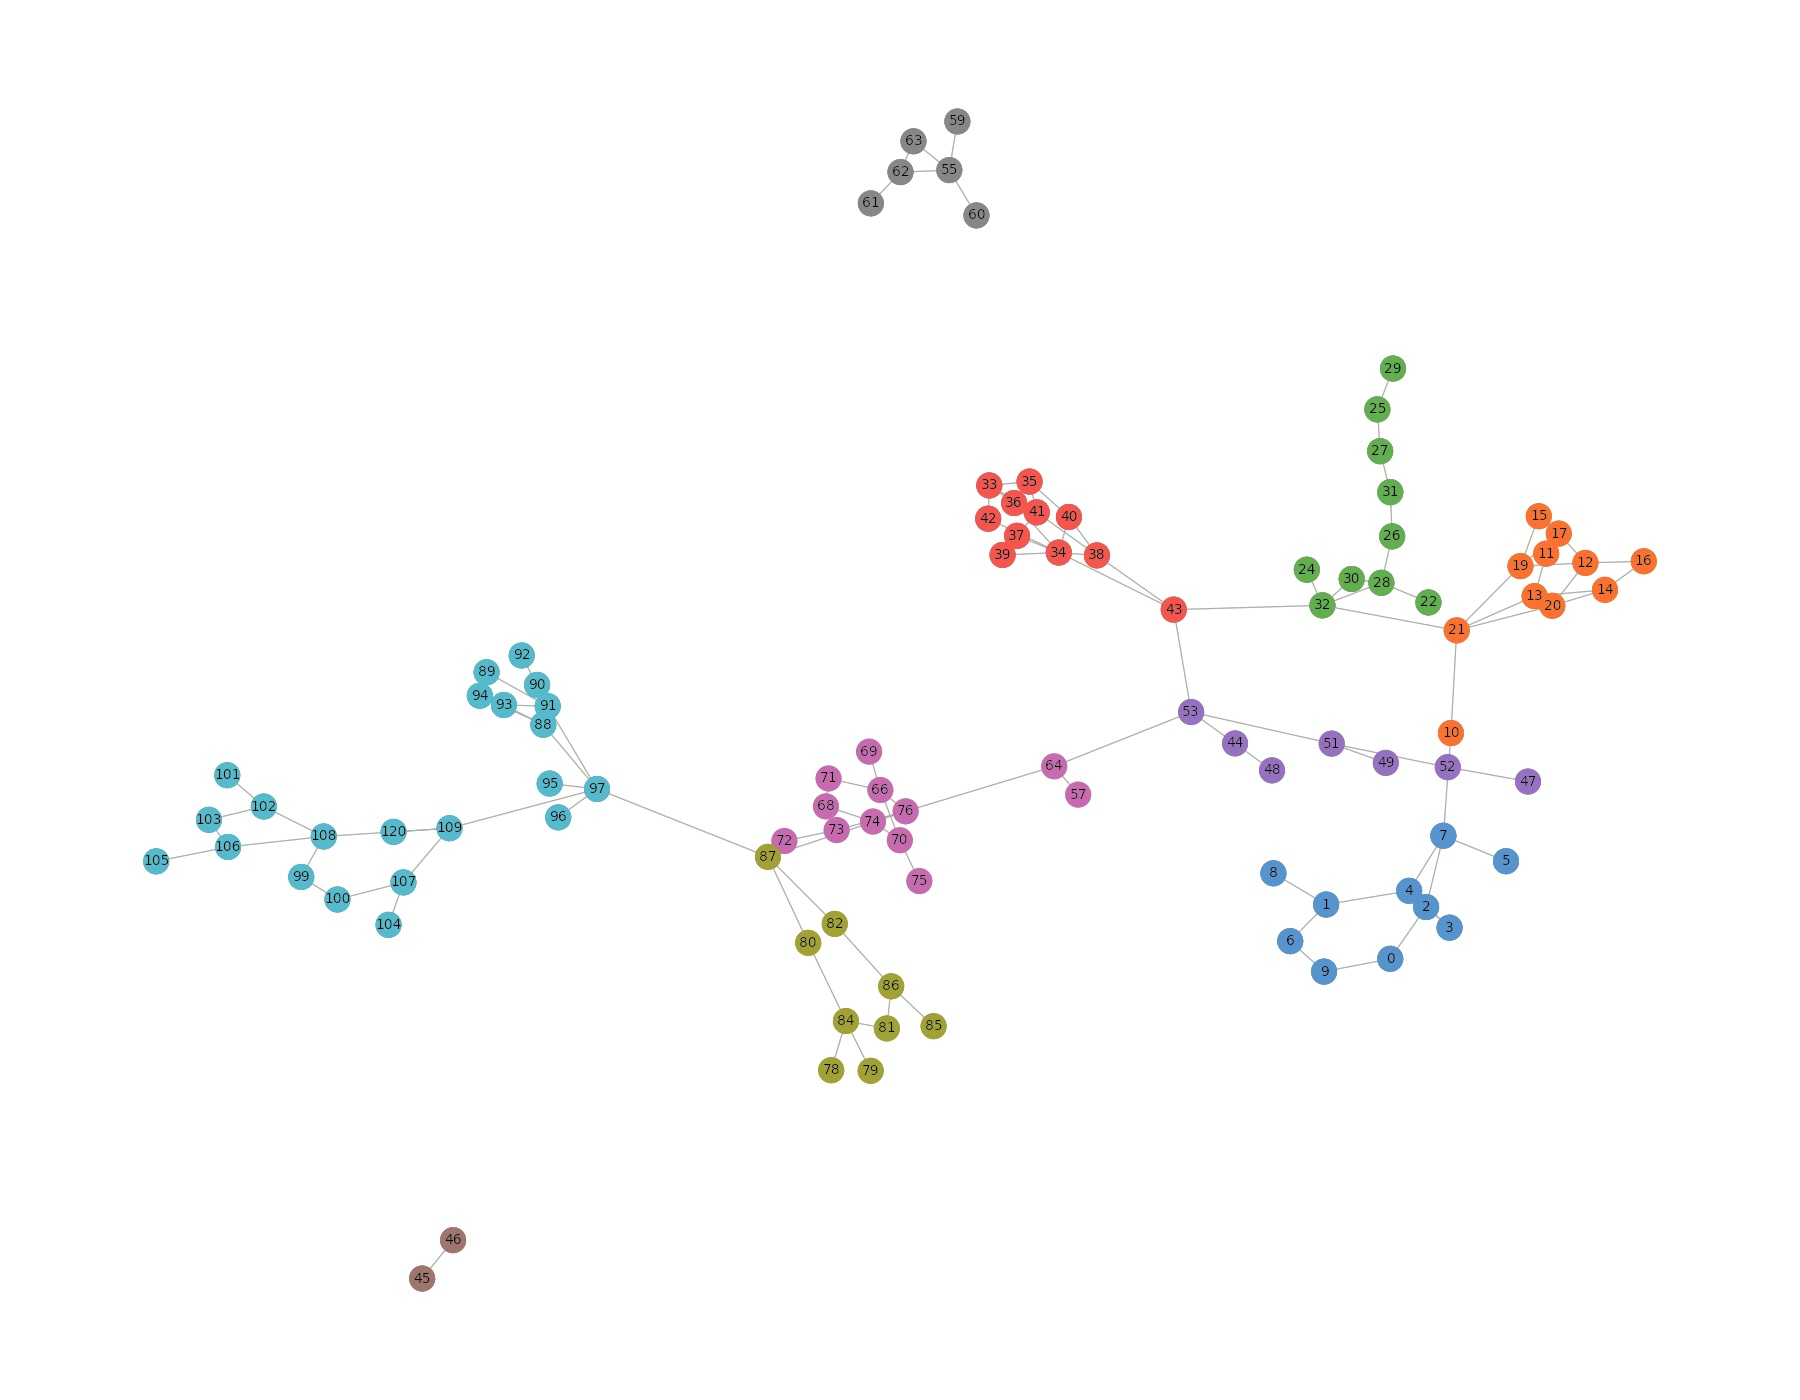
\includegraphics[width=1.0\textwidth]{Graphics/NearSocialNetwork.jpg}
    \caption{Zufälliger sozialer Graph mit höchster Grad-Zentralität als Verbindungsknoten }
    \label{NearSozialerGraph}
\end{figure}

\newpage
Nachdem Abbildung \ref{NearSozialerGraph} visuell betrachtet durchaus \textit{Sozialen Netzwerken} ähnelt, muss noch eine weitere Verbesserung durchgeführt werden. Bei einer genaueren Betrachtung der Abbildung fällt auf, dass die Teilgraphen wenige Verbindungen, Brücken, untereinander aufweisen. Dies liegt an der Idee von Algorithmus \ref{uniteGraphs}, den Knoten mit der höchsten Gradzentralität zu wählen und diesen dann mit einer beliebigen weiteren Gruppe zu verbinden. Doch in der Realität ist ein solches Phänomen sehr unwahrscheinlich und erfüllt nicht die Bedingungen aus Tabelle \ref{TableEigenschaften} für ein typisches soziales Netzwerk. Denn dies würde beispielsweise heißen, dass an der Universität Ulm alle Student(en)*innen der Fakultät für Ingenieurwissenschaften, Informatik und Psychologie untereinander in einer Weise miteinander verbunden sind, jedoch nur die Professor(en)*innen, welche die höchste Gradzentralität aufweisen, mit eine*m/r weiteren Professor*in einer anderen Fakultät verbunden sind. Dies ist aber nicht realistisch wenn bedacht wird, dass auch beispielsweise Student(en)*innen der Fakultät für Mathematik und Wirtschaftswissenschaften durchaus Kontakte zu der Fakultät für Ingenieurwissenschaften, Informatik und Psychologie haben können oder auch mit den jeweiligen Professor(en)*innen. Dementsprechend muss diese Eigenschaft ebenfalls in der Implementierung berücksichtigt werden. Das kann gewährleistet werden, indem jedem Knoten eine zufällige Wahrscheinlichkeit zugeschrieben wird, die angibt, ob eine Kante zwischen den Clustern oder Subgraphen existiert. Hierfür wird der Algorithmus \ref{uniteGraphs} ab Zeile \textit{17} ersetzt zu:

\begin{algorithm}
\caption{Verbindung Subgraphen}\label{connection}
\begin{algorithmic}[1]
\Procedure{connection subgraphs}{}
\State $\textit{prob} \gets \text{zufällige Zahl, die sehr klein ist}$
\For {alle \textit{i und j} liegen in der Matrix big graph}
\State \textit{befülle die Diagonale der Matrix mit 0}
\EndFor
\For {alle \textit{i und k} liegen in der Matrix}
\State $\textit{variable} \gets \text{zufällige Zahl zwischen 0 und 1}$
\If{\textit{variable} kleiner \textit{prob}}
\State \textit{setze big graph [i][k] auf 1}
\EndIf
\EndFor
\EndFor
\textbf{RETURN} big graph
\EndProcedure
\end{algorithmic}
\end{algorithm}

Mit Algorithmus \ref{connection} kann sichergestellt werden, dass die Subgraphen vermehrt miteinander verbunden sind und nicht von dem Knoten mit der höchsten Gradzentralität abhängen. Dadurch ist eine weitere Eigenschaft aus Tabelle \ref{TableEigenschaften} bezüglich der Existenz von mehreren Brücken, erfüllt.

\section{Die Analyse des generierten Graphen}
Mit den Überlegungen aus dem vorherigen Kapitel und den dort erläuterten Methoden, lassen sich \textit{typische soziale Netzwerke} nach den Eigenschaften von Tabelle \ref{TableEigenschaften} generieren. Um zu beweisen, dass es sich tatsächlich um ein typisches Netzwerk handelt, soll ein neues generiert und eine Analyse damit durchgeführt werden. Ziel ist es zu zeigen, dass die mit dem Generator erzeugten Graphen tatsächlich näherungsweise \textit{sozialen Netzwerken} entsprechen, welche die Bedingungen aus Tabelle \ref{TableEigenschaften}.

\FloatBarrier
\begin{figure}[h!]
    \centering
    \hspace*{-2cm}
    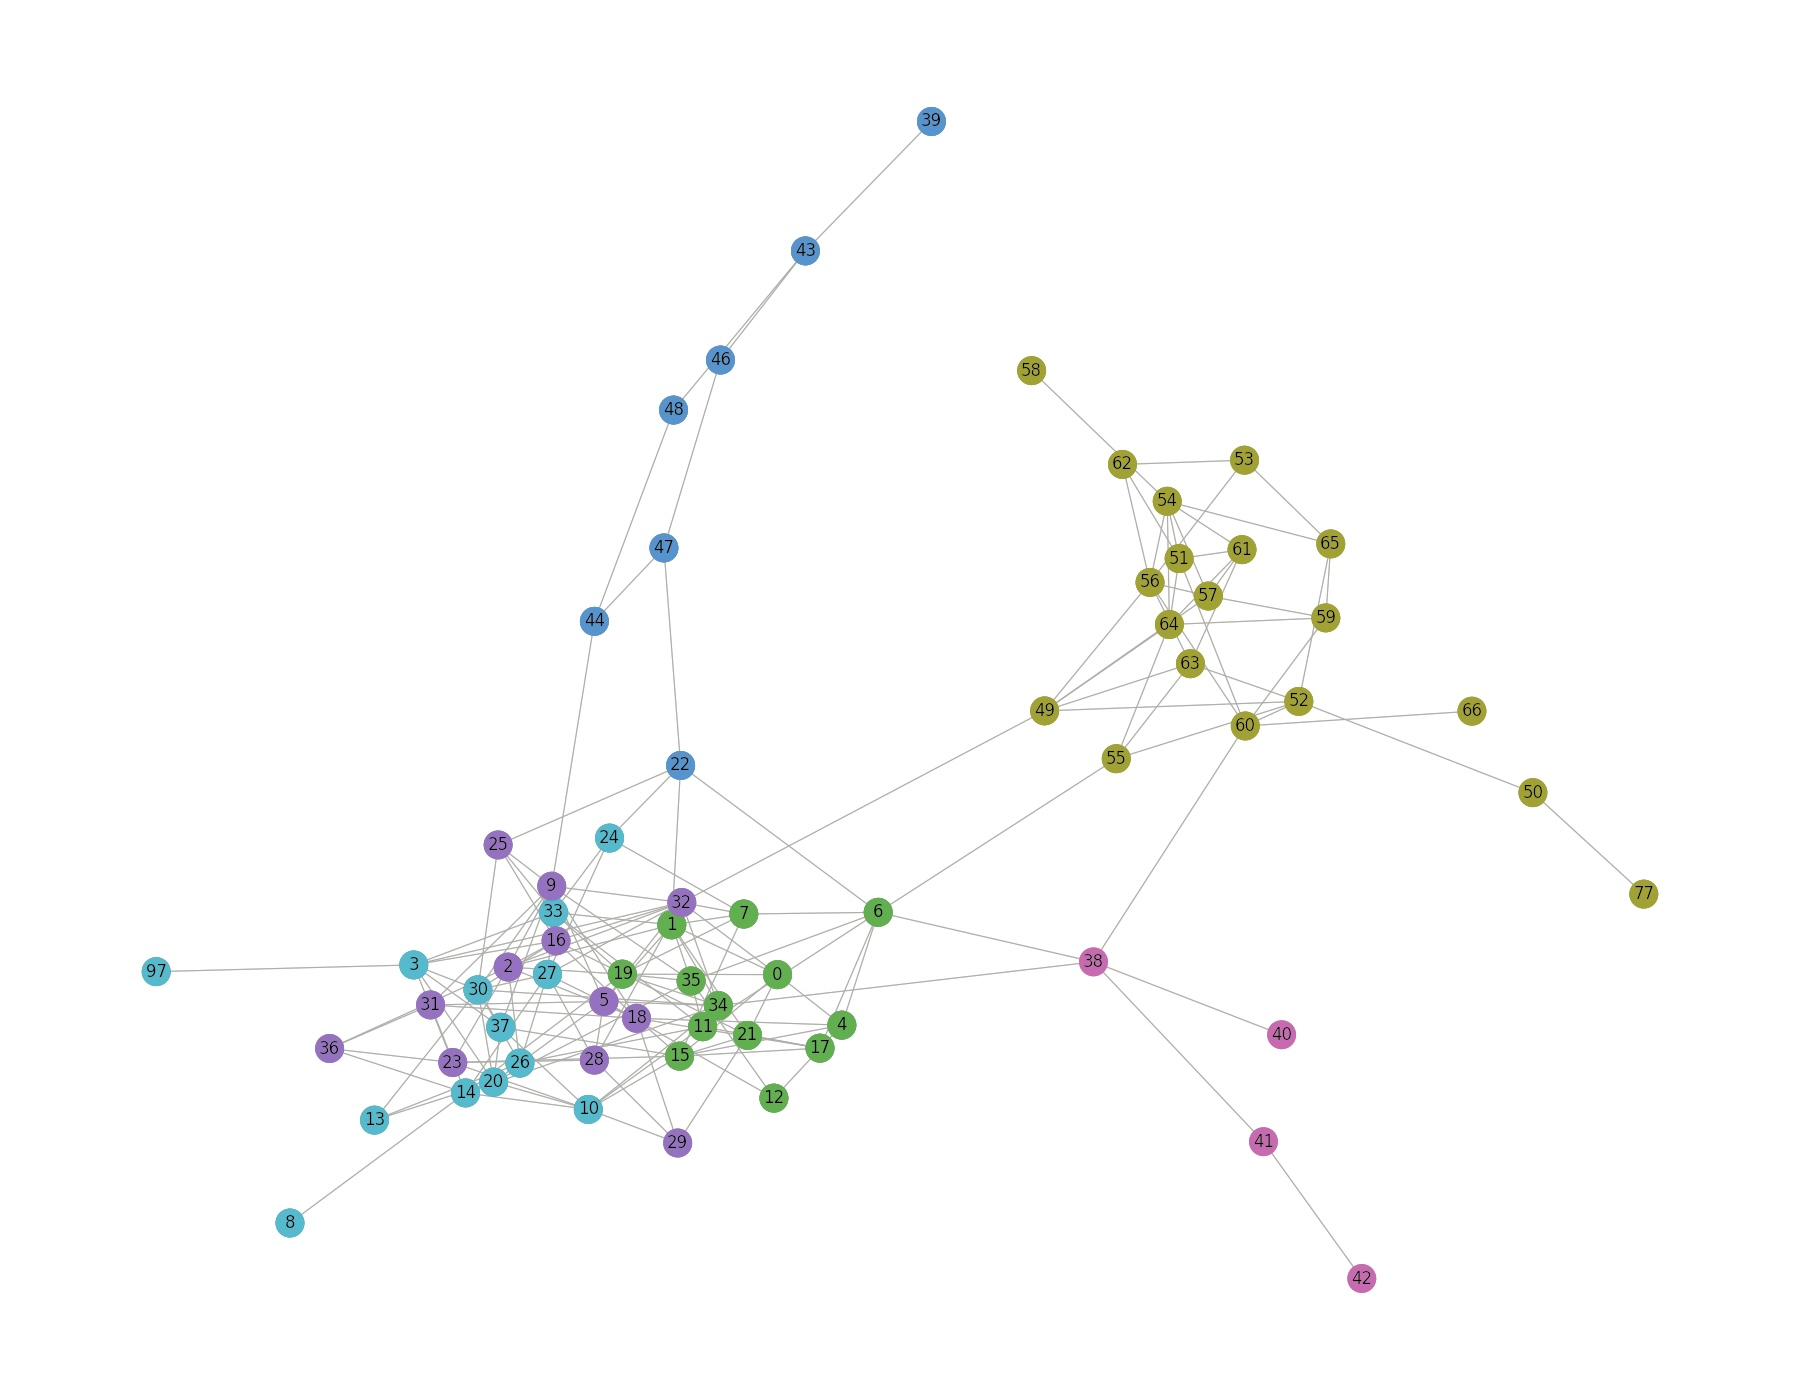
\includegraphics[width=0.7\textwidth]{Graphics/Random_moreConnections.jpg}
    \caption{Zufälliges soziales Netzwerk mit realistischeren Verbindungen}
    \label{fig:SNA}
\end{figure}

\FloatBarrier

Bei der visuellen Betrachtung der Abbildung \ref{fig:SNA} ähnelt die Struktur auf jeden Fall der, eines sozialen Netzwerks, siehe beispielsweise Abbildung \ref{fig:GameOfThrones}. Doch um eine fundierte Aussagen treffen zu können, müssen auch die Zentralitäten genauer analysiert werden. Hierfür wird folgende Tabelle verwendet:

\begin{table}[h!]
\footnotesize
\caption{Werte oberer Graph}
\begin{tabular}{lcccc}\toprule 
\textbf{Knoten} &\textbf{Grad-Zentr.} &\textbf{Nähe-Zentr.}  &\textbf{Between-Zentr.} \\
 &\\\midrule
  1 & 0.149254  & 0.389535 & 0.0429244   \\
  2 & 0.134328  & 0.370166 & 0.0366434   \\
  3 & 0.119403  & 0.350785 & 0.0516569   \\
  5 & 0.119403  & 0.378531 & 0.0341306   \\
  6 & 0.119403  & 0.385057 & 0.145038    \\
  7 & 0.0895522 & 0.358289 & 0.0208983   \\
 10 & 0.119403  & 0.341837 & 0.0240985   \\
 11 & 0.104478  & 0.360215 & 0.0212421   \\
 14 & 0.119403  & 0.3350    & 0.0454434   \\
 18 & 0.134328  & 0.340102 & 0.0283754   \\
 22 & 0.0746269 & 0.348958 & 0.0740623   \\
 27 & 0.119403  & 0.360215 & 0.0342121   \\
 30 & 0.149254  & 0.348958 & 0.0412278   \\
 32 & 0.179104  & 0.435065 & 0.266448    \\
 34 & 0.134328  & 0.394118 & 0.112543    \\
 35 & 0.104478  & 0.362162 & 0.0290967   \\
       
  \\\bottomrule
 \end{tabular}
  &
\begin{tabular}{lccc}
\toprule 
\textbf{Knoten} &\textbf{Grad-Zentr.} &\textbf{Nähe-Zentr.}  &\textbf{Between-Zentr.}\\
   &\\\midrule
 38 & 0.0746269 & 0.36612  & 0.154688    \\
 41 & 0.0298507 & 0.271255 & 0.0298507   \\
 43 & 0.0447761 & 0.198813 & 0.030303    \\
 44 & 0.0447761 & 0.295154 & 0.0773717   \\
 46 & 0.0298507 & 0.219672 & 0.0205638   \\
 47 & 0.0447761 & 0.27459  & 0.0520902   \\
 48 & 0.0298507 & 0.232639 & 0.0373285   \\
 49 & 0.0895522 & 0.36413  & 0.221288    \\
 50 & 0.0298507 & 0.241877 & 0.0298507   \\
 52 & 0.0895522 & 0.314554 & 0.0885577   \\
 54 & 0.104478  & 0.254753 & 0.0327816   \\
 55 & 0.0597015 & 0.325243 & 0.0670173   \\
 56 & 0.104478  & 0.303167 & 0.0672381   \\
 57 & 0.0746269 & 0.290043 & 0.0213757   \\
 60 & 0.0895522 & 0.313084 & 0.0903114   \\
 64 & 0.0895522 & 0.304545 & 0.0530434   \\
      \\\bottomrule
\end{tabular}
\end{table}
\label{TablleSNA}

\FloatBarrier
Bei dieser Tabelle handelt es sich um die \textbf{32} wichtigsten Knoten. Denn alle diese Knoten weisen eine höhere \textit{Zwischen-Zentralität} als \textbf{0.02} auf. Dieser Wert entspricht ungefähr dem Mittelwert aller berechneten Zentralitäten. Die andern Knoten sind außen vor gelassen, da sie in Relation gesehen eher unwichtig für das Netzwerk sind.
Bei der \textit{Grad-Zentralität} aus der Tabelle \ref{TablleSNA} sehen wir, dass die meisten Knoten einen Wert höher als \textbf{0.1} aufweisen. Zudem weisen einige, wenige Knoten eine \textit{Grad-Zentralität} höher als \textbf{0.13} auf. Genau genommen handelt es sich hier um Knoten \textbf{1} mit einem Wert von \textbf{0.149254}, Knoten \textbf{2} mit dem Wert \textbf{0.134328}, Knoten \textbf{18} mit dem Wert \textbf{0.134328}, Knoten \textbf{30} mit einer Zentralität von \textbf{0.149254}, zudem um Knoten \textbf{32} mit dem höchsten Wert von \textbf{0.179104} und schließlich Knoten \textbf{34} mit einer \textit{Grad-Zentralität} von \textbf{0.134328}. Die aufgezählten Knoten sind, den Werten zu urteilen nach, zentral wichtig für den Graphen und befinden sich höchstwahrscheinlich, visuell gesehen, im Zentrum des Graphen in Abbildung \ref{fig:SNA}. Bei der visuellen Analyse, kann diese Behauptung teilweise bestätigt werden, denn diese Knoten fallen direkt auf. Ein hoher Zentralitätswert bei einem Knoten sagt aus, dass es sich beispielsweise im realen Leben um eine vermutlich sehr berühmte / bekannte Person handeln wird. Daher besteht die Annahme, dass es sich bei diesem Knoten, würde er auf die Realität bezogen betrachtet werden, beispielsweise um einen Star, einen Influenzer oder eine, auf weitere Arten bekannte Person handelt. Doch ebenso ist es möglich, dass die Person viele weitere Personen kennt, oder von vielen weiteren Personen gekannt wird. Wichtig ist, dass nicht nur die Grad-Zentralität eine zentrale Rolle für die Analyse spielt. Im Weiteren betrachten wir auch die \textit{Nähe-Zentralität}. Doch um auch bei diesem Aspekt nicht alle \textbf{32} Werte aufzuzählen, werden im Folgenden nur Knoten betrachtet, die einen Wert höher als \textbf{0.37} aufweisen, da es sich dabei erneut um einen guten Mittelwert handelt. Diesen Grenzwert übertrifft der Knoten \textbf{1} mit einem Wert von \textbf{0.389535}, Konten \textbf{2} mit dem Wert \textbf{0.370166}, zudem Knoten \textbf{5} mit dem Wert \textbf{0.378531}, zusätzlich Knoten \textbf{6} mit der Zentralität \textbf{0.385057}, und schließlich Knoten \textbf{32} mit dem höchsten Wert von \textbf{0.435065} und \textbf{34} mit der Zentralität von \textbf{0.394118}. Laut der Definition aus dem Abschnitt \ref{ch:Zentralitaeten} gilt, je höher die Werte der \textit{Nähe-Zentralität} eines Knoten ist, desto näher befindet sich dieser Knoten zu weiteren Knoten bzw. weist die durchschnittlich kürzesten Wege zu diesen auf. Wird der Graph \ref{fig:SNA} anhand dieser Information betrachtet und werden so die Knoten mit der höchsten \textit{Nähe-Zentralität} gesucht, ist visuell ersichtlich, dass sich diese im gleichen Bereich befinden, wie die Knoten mit der höchsten \textit{Grad-Zentralität}. Die letzte zu untersuchenden Zentralität ist die \textit{Betweenness-Zentralität}. Auch hier betrachtet man wieder die Knoten mit den höchsten Werten, und um nicht alle \textbf{32} Werte aufzuzählen, werden erneut nur Knoten mit einem Wert höher als \textbf{0.09} ausgewählt. Diese Voraussetzung erfüllen neben dem Knoten \textbf{6} mit dem Wert \textbf{0.145038} die Knoten \textbf{32} mit der höchsten Zentralität von \textbf{0.266448} und \textbf{34} mit einem Wert von \textbf{0.112543}, außerdem der Knoten \textbf{38} mit der Zentralität von \textbf{0.154688}, zudem der Knoten \textbf{49} mit dem Wert \textbf{0.221288} und schließlich der Knoten \textbf{60} mit dem Wert \textbf{0.0903114}. Das bedeutet für unseren Graphen in Abbildung \ref{fig:SNA}, dass die kürzesten Wege anteilsmäßig am öftesten über diese genannten Knoten verlaufen. Zudem kann vermutet werden, dass es sich bei diesen Knoten um \textit{Brücken} handelt, was der Behauptung aus dem vorherigen Kapitel \ref{ch:CliquenBrücken}, dass es sich bei hohen \textit{Zwischen-Zentralitäten} um \textit{Brücken} handelt, bestätigen würde. Bei der erneuten Betrachtung des Graphen, erkennt man nämlich, dass sich die Knoten in den grün, lila, hellblauen Teilgraphen befinden und links unten zentriert sind. Doch kommt bei der \textit{Zwischen-Zentralität} hinzu, dass sich die Knoten \textbf{49} und \textbf{60} auch im gelbgrünen, rechts oben liegenden, Teilgraphen befinden. Außerdem ist auf den ersten Blick zu erkennen, dass es sich bei den 6 Knoten in Abbildung \ref{fig:SNA} visuell betrachtet, tatsächlich um Brücken handelt. Im Allgemeinen ist es eindeutig, dass die Werte gut zu den bisher generierten Plots passen und es sehr wahrscheinlich ist, dass die Annahme korrekt ist und die Knoten tatsächlich am häufigsten bei allen kürzesten Wegen durchlaufen werden und tatsächlich Brücken sind. Leider ist die Anzahl an \textit{Cliquen} des Graphen aus der Abbildung \ref{fig:SNA} nicht mehr exakt bekannt, da erst nach der weiteren Verbesserung des Codes Rücksicht drauf genommen wurde, die Cliquen-Größe und -Anzahl direkt vorzugeben. Daher wird an dieser Stelle nur die Vermutung aufgestellt, dass alle Knoten aus der Tabelle \ref{TablleSNA} Teil von Cliquen sind. Wie viele es jedoch genau sind, lässt sich an dieser Stelle leider nur wage vermuten. Im nächsten Abschnitt wird zusätzlich die Betrachtung der Cliquen des Graphen mit einbezogen. Weitere Zentralitätswerte und Eigenschaften des Graphen werden an dieser Stelle nicht betrachtet. Nachdem alle Kriterien aus Tabelle \ref{TableEigenschaften} überprüft sind und erfolgreich festgestellt wurde, dass dieser Graph einem \textit{sozialen Netzwerk} ähnelt, wird noch ein weiterer Graph generiert, um sicherzustellen dass es sich nicht um eine zufällige Übereinstimmung handelt. An dieser Stelle soll auch noch ein weiteres Kriterium untersucht werden, nämlich die Verteilung der Zentralitäten.


\newpage
\section{Die Verteilung der Zentralitäten}
Nachdem im vorherigen Kapitel die Generierung eines \textit{sozialen Netzwerkes} und die Analyse durchgeführt wurde, spielt im Folgenden die Verteilung der Zentralitätswerte eine wichtige Rolle.
Im Laufe der Arbeit ist aufgefallen, dass sich die Werte der Zentralitäten, von den bisher generierten Graphen, oftmals in einem ähnlichen Wertebereich befinden. An dieser Stelle kommt die Frage auf, wie diese Werte verteilt sind und ob die Verteilung möglicherweise einer mathematischen Wahrscheinlichkeitsverteilung entspricht beziehungsweise ähnelt. Das heißt im Konkreten, es wird der Frage nachgegangen, ob alle Zentralitätswerte sozialer Netzwerke ähnliche Verteilungen nachweisen. Wenn sich die Vermutung bestätigt, können andere soziale Netzwerke anhand dieses Kriteriums verglichen werden.
Erdös und Renyi (1960), Cliff und Ord (1973) und Friedkin (1981) arbeiteten bereits an Zufallsgraphen und haben die Definition erstellt, dass alle Graphen mit $N$ Knoten und $E$ Kanten dieselbe Wahrscheinlichkeiten haben, ausgewählt zu werden. Ein bekanntes Ergebnis von Erdös und Renyi (1960) ist zudem, dass die Zentralitäten, vor allem aber die Grad-Zentralität, hypergeometrisch verteilt ist, was durch eine Poisson-Verteilung angenähert werden kann \cite{Distribution}. Weitere, vor allem mathematische Beweise, können dem Buch \cite{Distribution} entnommen werden. Im weiteren Teil dieser Arbeit wird demnach untersucht, ob die Verteilungen der Zentralitäten der \textit{Poisson-Verteilung} ähnelt. Zu der \\ Tabelle \ref{TableEigenschaften} kommt also eine weitere, letzte Zeile hinzu:

\begin{table}[h!]
\footnotesize
\caption{Weitere Eigenschaft eines sozialen Netzwerks}
\label{TableEigenschaften2.0}
\centering
\begin{tabular}{lcc}\toprule 
\textbf{Eigenschaft} &\textbf{Beschreibung} \\
 &\\\midrule
 \\
  \textbf{Verteilung der Zentralitäten} & die Zentralitäten eines soziales Netzwerk sollten \\ &annähernd einer Poisson-Verteilung entsprechen \cite{verteilung} \\
  \\\bottomrule
 \end{tabular}
 \end{table}

Da der Graph in Abbildung \ref{fig:SNA} ein zufällig, einmalig erzeugter Graph ist, muss ein neuer Graphen mithilfe des Generators erzeugt werden, um die Verteilung der Zentralitäten zu betrachten. Dies wird sich nicht auf die Untersuchung auswirken, denn die Verteilungen der Zentralitäten unserer Graphen sollte stets gleich oder zumindest ähnlich sein. Bei der erneuten Generierung entsteht nun folgender Graph \ref{fig:distribution} und die zugehörige Verteilung der \textit{Grad-Zentralität}:

\FloatBarrier
\begin{figure}[h!]%
  \centering
  \subfloat[][]{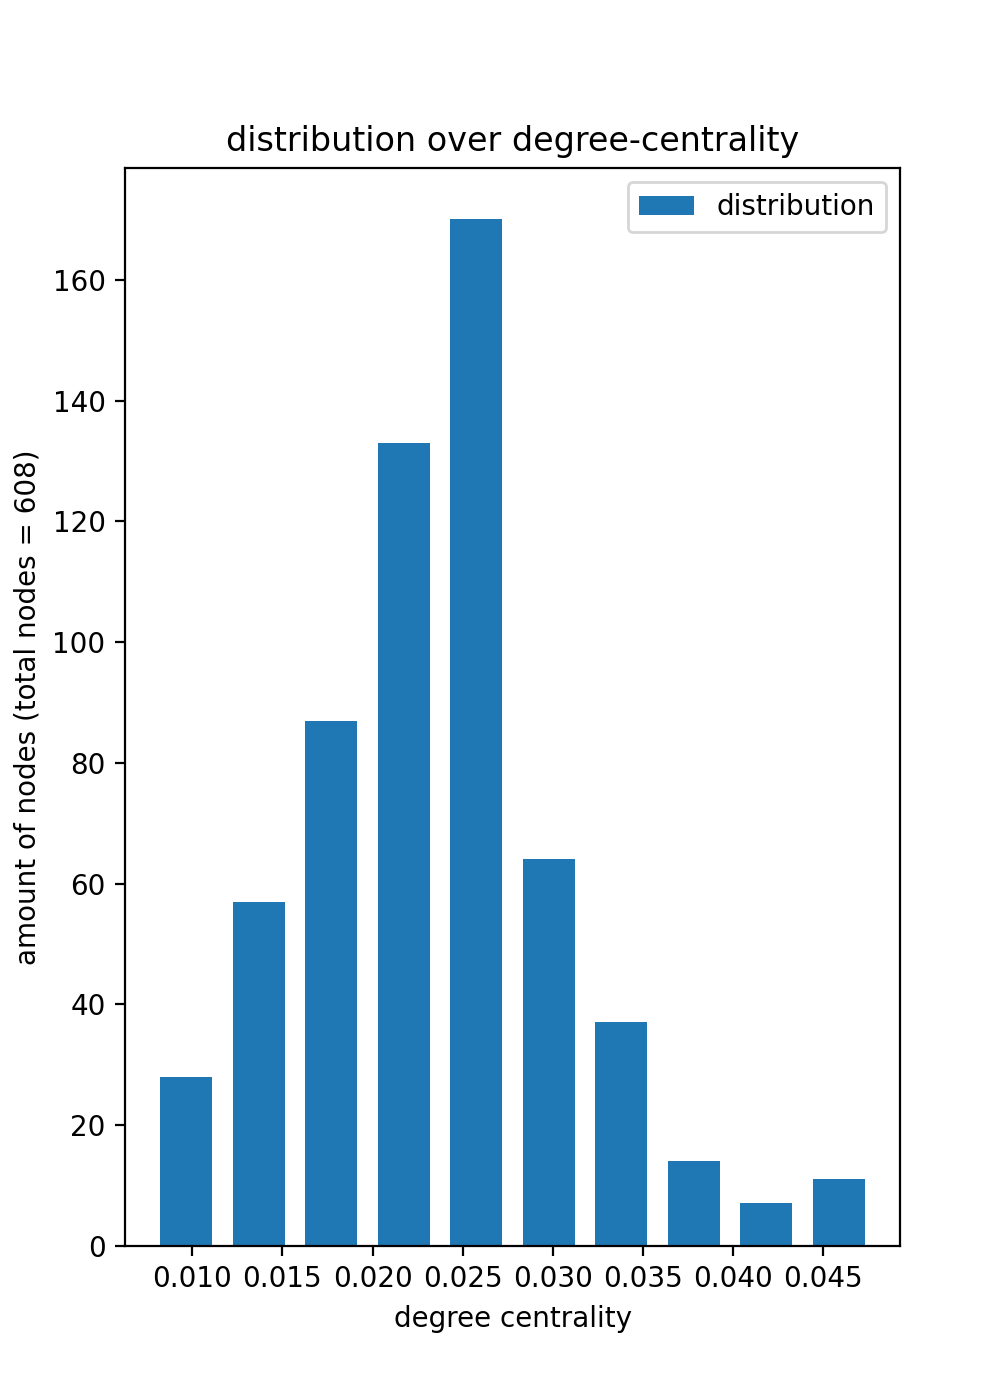
\includegraphics[width=0.4\linewidth]{Graphics/distribution_degree.png}}%
  \qquad
  \subfloat[][]{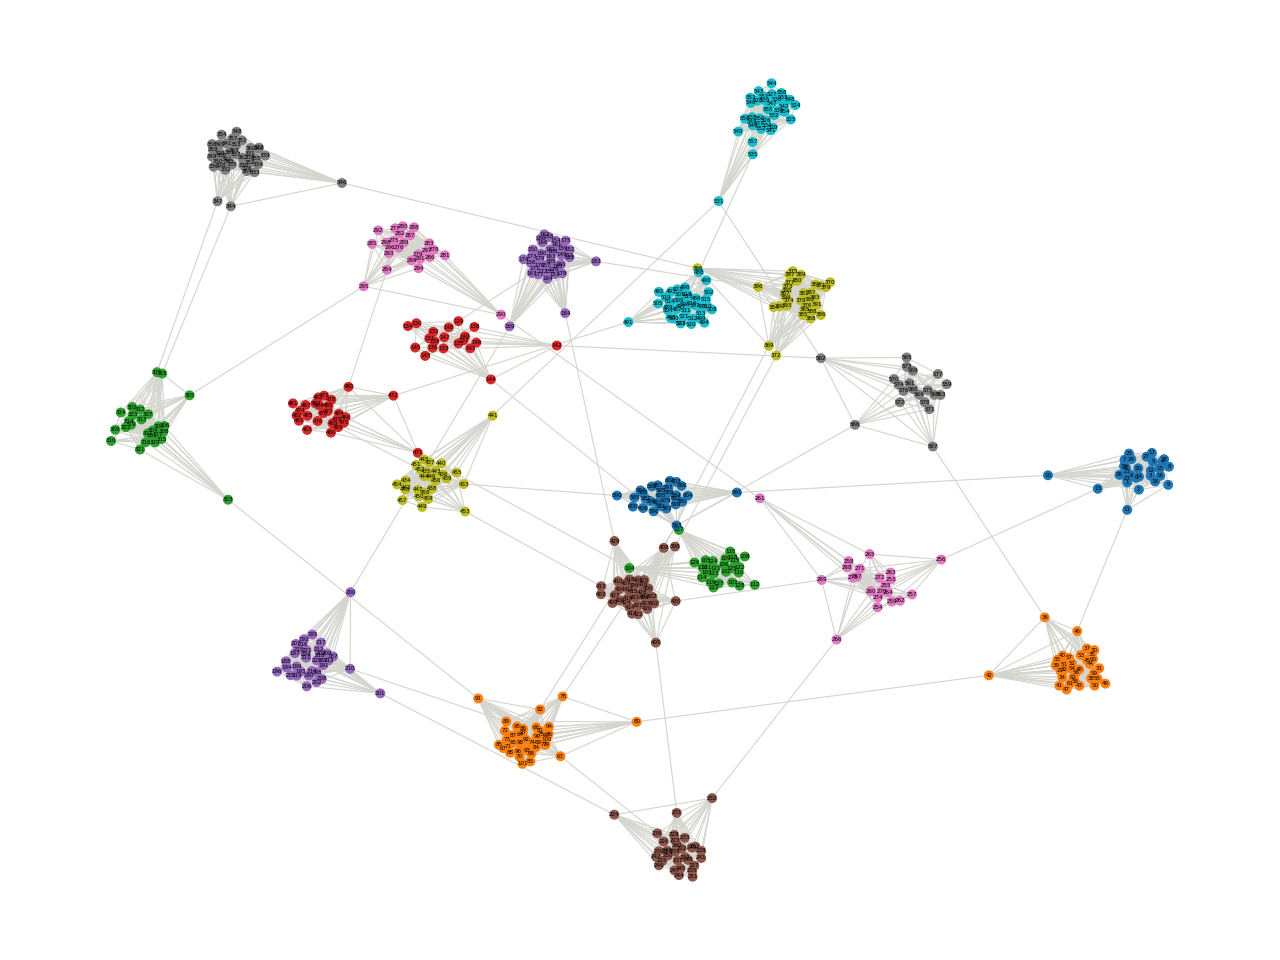
\includegraphics[width=0.5\linewidth]{Graphics/plot_degreeDist.png}}%
  \caption{Verteilung der Grad-Zentralität des Graphen (b)}%
  \label{fig:distribution}
\end{figure}
\FloatBarrier

Es wird ersichtlich, dass die \textit{Grad-Zentralität} normal- beziehungsweise gaußverteilt ist. Natürlich ist zu erwähnen, dass keine perfekte Normal-Verteilung zu sehen ist, sondern eine etwas nach links verschobene Verteilung. Was die möglichen Gründe dafür sind, werden später betrachtet und korrigiert. Diese Verteilung erfüllt tatsächlich die Eigenschaft aus \\
Tabelle \ref{TableEigenschaften2.0}, denn die Poisson-Verteilung wird für ein größer werdendes $\lambda$ zu einer gaußschen Normalverteilung \cite{Poisson}. Nun ist aber auch noch zu untersuchen, ob sich die Eigenschaft, der  poisson verteilten Zentralitäten, für die \textit{Nähe-} und \textit{Zwischen-Zentralität} ebenfalls beobachten lässt. Um zusätzlich zu beweisen, dass es sich bei der Gauß-Verteilung der Werte nicht um einen Zufall handelt, wird ein neuer sozialer Graph generiert und die Verteilung der \textit{Grad-}, \textit{Nähe-}, \textit{Zwischen-} und \textit{Eigenvektor-Zentralität} untersucht. Hierbei ist vor allem die Frage, ob die Verteilung dieser einer tatsächlichen Poisson-Verteilung entspricht und falls ja, warum dies der Fall ist, essentiell. Ansonsten wird die Frage gestellt, warum es keiner Poisson-Verteilung entspricht und ob es möglich ist, den Graphen zu verändern um eine solche zu erzielen. Bei der erneuten Generierung entstehen schließlich folgende Plots:

\FloatBarrier
\begin{figure}[h!]%
  \centering
  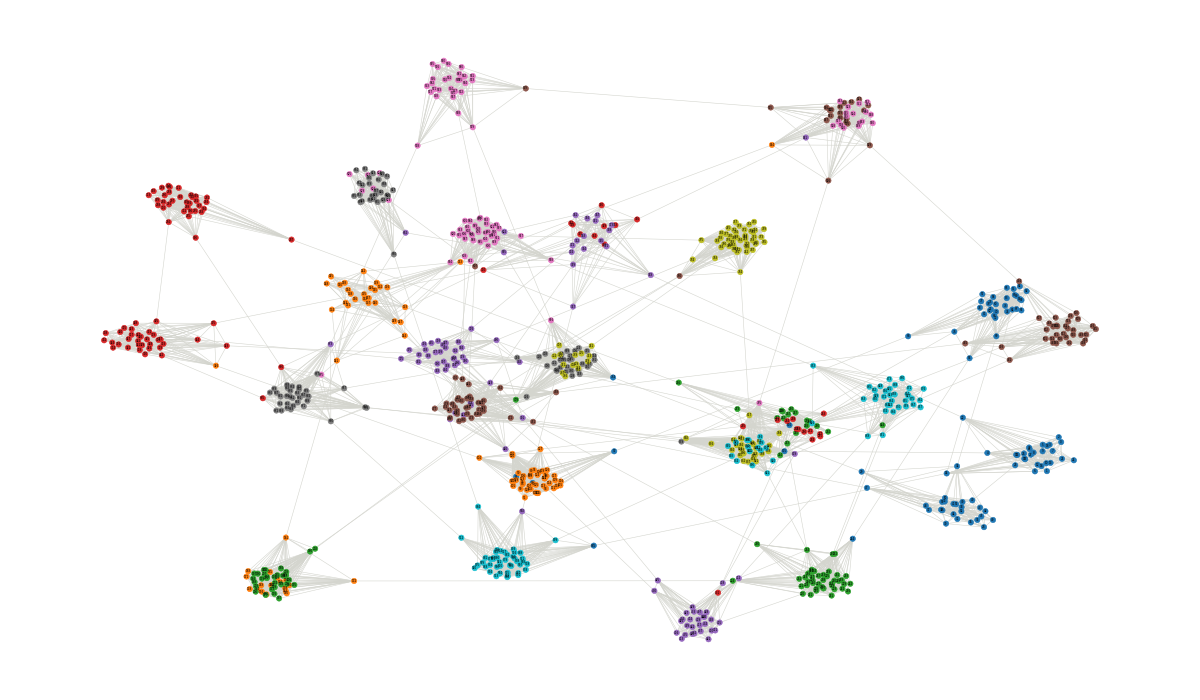
\includegraphics[width=0.7\textwidth]{Graphics/newourSN.png}
  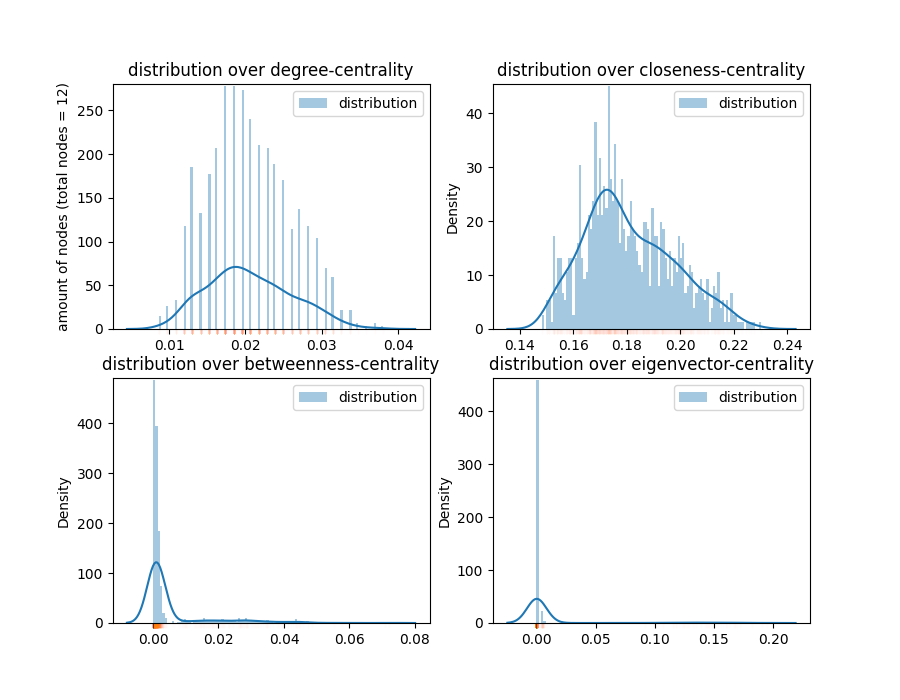
\includegraphics[width=0.9\textwidth]{Graphics/newOurDist.png}
  \caption{Zufälliges soziales Netzwerk und realistischeren Verteilungen}
  \label{fig:distributionALL}
\end{figure}
\FloatBarrier
In der Abbildung \ref{fig:distributionALL} sieht man nun die Verteilungen der Zentralitäten von dem, sich darüber befindenden, sozialen Netzwerks. Die Tabelle mit den Zentralitäts-Werten des Netzwerks befindet sich als Datei in \cite{TZ}. Oben links befindet sich die Verteilung der \textit{Grad-Zentralität}, welche wie bereits zuvor festgestellt, nicht exakt normalverteilt ist, aber Ähnlichkeiten zu erkennen sind und demnach ebenfalls eine annähernde Poisson-Verteilung zu erkennen ist. Vor allem ist auffällig, dass der Balken bei \textbf{0.012} vergleichsweise sehr hoch ist. Über \textbf{50} Knoten weisen diesen Wert auf. Danach geht der darauf folgende Balken nochmals zurück, denn nur noch etwas über \textbf{25} Knoten haben eine Zentralität von circa \textbf{0.03}. Jedoch war zu erwarten, dass sich das Balkendiagramm symmetrisch verhält um der mathematischen Verteilung zu entsprechen, doch das Gegenteil tritt ein. Der genaue Grund hierfür ist mir nicht ersichtlich, aber besteht die Vermutung, dass es nicht weiter schlimm ist und es ausreicht, dass die Verteilungen lediglich annähernd der Poisson-Verteilung entsprechen. Über \textbf{150} Knoten weisen eine Zentralität von \textbf{0.0125} auf, daher sollten auch ebenso viele den Wert \textbf{0.025} besitzen. Hingegen ist positiv hervorzuheben, dass genau \textit{ein Peak} erreicht wurde, wie auch zu erwarten war, um der mathematischen Verteilung zu entsprechen. Außerdem sind alle Balken vor dem Peak kontinuierlich aufsteigend und nach dem Peak kontinuierlich absteigend. Doch lediglich eine Unstimmigkeit sticht hier heraus, bei dem Zentralitätswert von \textbf{0.0357} den etwas unter \textbf{25} Knoten besitzen. Fraglich ist hier, warum der Balken erneut höher ist als sein Vorgänger. Denn im Regelfall sollten maximal ein bis drei Knoten gefunden werden, die diesen Wert aufweisen. Doch im Allgemeinen weist der Plot genau die Eigenschaft nach, die auch zu erwarten ist, nämlich dass die \textit{Grad-Zentralität} annähernd poisson verteilt ist.\\

Das Balkendiagramm der \textit{Nähe-Zentralität} weist einen ähnlichen Verlauf auf wie das der \textit{Grad-Zentralität}. Wir erkennen erneut das erwartete Peak und weitere Balken, die im linken Bereich sehr schnell zum Peak hin ansteigen und rechts vom Peak vergleichsweise langsam abflachen. Auffällig ist erneut, dass der letzte Balken wider Erwartens höher ist als der Balken davor. Eine Aussage, welche auf jeden Fall getroffen werden kann ist, dass es erneut zu Unstimmigkeiten kommt, welche stets an anderen Stellen auftreten und nicht immer denselben Balken betreffen. Doch ist erneut eine Normal Verteilung zu erkennen, die der Poisson Verteilung für hohes $\lambda$ entspricht \cite{Poisson}. Es kann im Allgemeinen zudem angenommen werden, dass je größer der Graph ist, umso eher sind die Zentralitäten von diesem poisson verteilt. Was daran liegt, dass dieser dann mehr Knoten besitzt und diese irgendwann zwangsläufig eine Regelmäßigkeit aufzeigen, da Zahlen in der Mathematik prinzipiell nicht \textit{zufällig}, sondern normalverteilt sind. Grob zusammengefasst, kann die Existenz einer Kante als Binomialverteilung interpretiert werden und diese konvergiert mathematisch gesehen bei einer sehr großen Stichprobe (Anzahl an Knoten in unserem Fall) gegen eine Normal- bzw Gaußverteilung. \\

Bei der \textit{Zwischen-} und \textit{Eigenvektor-Zentralität} sind andere Verteilungen zu erkennen. Zum einen weisen die Balken wenige unterschiedliche Werte auf, zum anderen sind die Ausschläge nicht mehr mittig sondern direkt zu Beginn der Verteilung. Was zunächst verwunderlich erscheint, ist mit einer simplen Erklärung begründet. Die \textit{Nähe-Zentralität} gibt bekanntlich an, wie oft ein Knoten anteilsmäßig bei der Suche nach dem kürzesten Weg durch einen Graphen benutzt wird. Der Ausschlag ist daher die Folge davon, wenn viele kürzeste Wege stets über die gleichen Knoten verlaufen. Das heißt, es existieren keine bis wenige Alternativen und daher verlaufen die kürzesten Wege von beispielsweise Knoten \textbf{1} zu einem weiteren Knoten stets über gleiche, beziehungsweise ähnliche Knoten. Bei der \textit{Eigenvektor-Zentralität} wird zwar die gleiche Beobachtung gemacht, doch sagt diese hier etwas anderes aus. Diese Zentralität gibt eine Einschätzung der Wichtigkeit des Knotens, im Bezug auf seine Nachbarn an, was bezogen auf die Balkendiagramm heißt, dass viele Knoten in diesen Graphen wichtig sind mit Einbeziehung der Nachbarn. Wobei auch vermuten werden darf, dass dies mit der hohen Anzahl an Konten mit höher \textit{Zwischen-Zentralität} zusammenhängt.\newpage
Das heißt im Umkehrschluss wiederum, dass mehr Cliquen im Graph enthalten sind. Tatsächlich sind es \textbf{935} Knoten, \textbf{8952} Kanten und \textbf{10301} Cliquen mit der maximalen Größe von acht Knoten in der Clique.
Die Verteilungen sind dennoch aus der Mathematik bekannt, denn es handelt sich um die \textit{Exponential-Verteilung}, welche ebenfalls in eine \textit{Poisson-Verteilung} übergehen kann. Wie dies genau funktionier, ist \cite{PoissonMathepedia} zu entnehmen.
Danach zu Urteilen handelt es sich bei dem Netzwerk in Abbildung \ref{fig:distributionALL} um ein typisches \textit{soziales Netzwerk} nach Tabelle \ref{TableEigenschaften} und Tabelle \ref{TableEigenschaften2.0}.

\section{Kurzes Recap}
Nachdem zunächst überlegt wurde, wie soziale Netzwerke generiert werden, sind auch gleichzeitig die Probleme der Generierung aufgefallen. Daher wurde der Code fortlaufend verbessert, ein soziales Netzwerk erstellt und danach eine \textit{soziale Netzwerk Analyse} durchgeführt. Schließlich konnte so die Bestätigung erhalten werden, dass die generierten Graphen die Anforderungen eines sozialen Netzwerks aus den Tabellen \ref{TableEigenschaften}, \ref{TableEigenschaften2.0} erfüllt. Danach ist zudem aufgefallen, dass die Zentralitäten regelmäßig sind und eine Poisson-Verteilung nachgewiesen werden kann. Doch muss im Folgenden noch die Frage beantwortet werden, wie die Verteilung der Zentralitäten bei anderen, bereits analysierten, Netzwerken aussieht.
